\documentclass[10pt,letterpaper]{book}
\usepackage[latin1]{inputenc}
\usepackage{amsmath}
\usepackage{amsfonts}
\usepackage{amssymb}
\usepackage[pdftex]{graphicx}
\author{Christopher C. Lamb, Pramod A. Jamkhedkar, Gregory L. Heileman}
\title{Usage Management in the Cloud}
\begin{document}
\maketitle
\tableofcontents
\chapter{Usage Management in the Cloud}
\section{Introduction}
The characteristics of cloud computing services tend to differ from those of grid and cluster-based computing applications.  Specifically, cloud services tend to be more market oriented, and they typically host entire user applications within the distributed cloud environment. These characteristics raise serious concerns from cloud users' perspective regarding the manner in which their data are handled or used by the cloud services. These metrics are orthogonal to the traditional performance-oriented quality of service (QoS) metrics, and their semantics are well beyond encryption and privacy requirements. Existing service level agreement (SLA) frameworks focus primarily on performance-oriented QoS parameters, and are not designed for expressing and enforcing policies to control the manner and restrictions under which users' data need to be handled~\cite{WSA, WSLA, WSP,PaRaSh:09}. User concerns on data handling in the cloud along with the limitations of existing SLA frameworks to express, reason and enforce data usage policies in an automated manner creates the need for usage management in cloud computing. 
 
Usage management is the collective set of processes and mechanisms that enables one to manage and control how data are
used within a system. This encompasses policy specification languages, licensing mechanisms, policy expression and reasoning mechanisms, policy enforcement mechanisms, usage tracking, along with supporting authentication and encryption mechanisms~\cite{PaSa:04,JaHeLa:10}. The ability to express fine-grained usage policies will provide cloud users with greater trust regarding the usage of their data within clouds, and will provide them with the confidence to employ cloud services. A mechanism to interpret, reason over, and enforce usage policies within clouds in an automated manner will allow cloud providers to optimize resource allocation while ensuring safety and security of cloud users' data. A correct estimation of the cost involved in enforcing usage policies will further enable cloud providers with business opportunities such as yield management and price differentiation. 

This paper introduces the notion of usage management in cloud computing and provides an in-depth analysis of the challenges and principles involved in the design of an open, interoperable usage management framework that operates over a distributed cloud computing environment. The analyses include application of well-known principles of system design and standards~\cite{BlCl:01,Cl:88,ClWrSoBr:02}, research developments in the areas of usage control~\cite{PaSa:04,JaHeLa:10}, policy languages design principles~\cite{JaHeMa:06}, digital rights management (DRM) systems~\cite{JaHe:09},  and interoperability~\cite{JaHe:04,HeJa:05,KoLaMaMi:04} towards the development of such a framework.

The paper delves into how such a framework will improve upon the status quo by leveraging  existing security mechanisms, and enabling automated reasoning of policies with respect to the underlying cloud security infrastructure. Based on these analyses, a system for expressing and reasoning about usage management within a distributed cloud environment is proposed that makes use of a common cloud ontology shared by different cloud services. The proposed system architecture enables usage policies to be expressed in different policy languages, and interpreted across various cloud environments. 

The remainder of the paper is structured as follows. Section~\ref{sec:motivation} introduces the need for incorporating usage management in cloud computing. An analysis of the features of a usage management framework for cloud computing environments is provided in Section~\ref{sec:clouds-usage}. In Section~\ref{sec:architecture} a preliminary architecture for usage management is proposed that makes use of a common cloud ontology and enables use of multiple policy languages. We then move into the challenges associated with scaling these kinds of solutions to cloud environments, and then close the chapter.

\section{Motivation and Related Work}\label{sec:motivation}
In the recent years, cloud computing has  managed to emerge as a computing platform that allows computing services to be consumed as a utility by consumers. In cloud computing, applications, systems software, and hardware are offered as utility services to consumers over the Internet. In service-based architectures, service consumers need to be provided with  highly reliable services that meet their expectations. Service consumers indicate these expectations in terms of QoS parameters that are expressed in the form of an SLA negotiated with the service provider. 

In the realm of computing, there exist multiple service-based paradigms such as web-services, cluster computing, grid computing and cloud computing~\cite{Bu:09}. Cloud computing is set apart from the other forms of service-based computing paradigms by a collective set of distinguishing characteristics such as market orientation, virtualization, dynamic provisioning of resources and service composition via multiple service providers~\cite{BuYeVeBrBr:09}. These characteristics imply that in cloud computing,  cloud users' data reside in the cloud for a finite amount of time, that these data are handled by multiple cloud services, and that data fractions may be stored, processed, transformed and routed across a geographically distributed cloud infrastructure. These activities occur ``behind-the-scenes'', within the cloud, while giving cloud users an impression of a single virtual machine.  In current cloud implementations,  cloud users have very little control over the manner in which data are handled by cloud providers, once they are pushed into the cloud. As consumers start aggressively using cloud services, this limitation will become a matter of serious concern. 

The handling or use of cloud users' data within the cloud by different services refers to policies specifying the constraints under which different actions may be carried out on the data. A cloud user may want to limit the manner in which data are stored, routed, or processed, and specify the entities and processes that are authorized to carry out these activities, and under what conditions. As an example, a government agency might want to prevent its data from being stored in one particular country, or prevent routing of the data via a particular set of networks it considers unreliable or insecure. Similarly, a financial company might want to prevent its data from being processed by a particular cloud service, or may want the data to be encrypted before being stored by an untrusted cloud storage service. Usage policies typically consist of a range of semantics such as restrictions on the manner in which data are used, temporal restrictions on usage, spatial or attribute-based restrictions, permissions, obligations, penalties, count-based limits on usage, usage tracking and reporting, and partial dependencies to name a few.   Hence, as cloud services become pervasive, cloud users will want to dictate the terms of usage for their data within the cloud in a manner that is expressive enough to capture their concerns. 

Existing cloud infrastructures and SLA frameworks are ill-equipped to address the requirements and challenges of usage management in distributed cloud systems. At present, cloud providers enable usage management features via rudimentary techniques involving a  one-size-fits-all option, where cloud users have little or no say in expressing usage policies over their data. For example, the Amazon S3 storage service allows a region-based facility where data stored in one region are guaranteed not to leave that particular region~\cite{AWS}. Such options are too coarse and simplistic to address cloud users' concerns. 

Existing service-based computing paradigms such as web services, clusters and grid computing use well-established SLA frameworks that enable expression, interpretation, monitoring, control and enforcement of SLA terms~\cite{WSA, WSLA, WSP,PaRaSh:09}. However, the SLAs supported by these frameworks focus on performance metrics such as availability, reliability, bandwidth, response times, instructions per second, etc. ~\cite{PaSc:06}. Also, the privacy and security metrics supported by these frameworks focus primarily on encryption of data. Performance-based metrics are end-to-end, meaning that users are concerned only with the delivery of performance, and not about the measures taken by service providers to deliver the service. The service provider simply maintains the required quality of service by allocating more resources or employing additional third party services. Compared to this, usage management requirements are different since cloud users potentially have a say in every action taken on their data, throughout the lifetime of the data in the cloud, including scenarios where the data are passed on to a third party provider. 

Usage management requirements are significantly different from QoS-based metrics, and present a new set challenges that are beyond the capabilities of the existing SLA frameworks. It is therefore necessary to design a separate mechanism for usage management that will enable persistent, automated management data usage control, while allowing seamless flow of data in a distributed cloud infrastructure. 

\section{Usage Management in Clouds}\label{sec:clouds-usage}
There exists a rich body of research in the areas of access control~\cite{BlPa:73,BlPa:76}, usage control~\cite{PaSa:04,JaHeLa:10} and DRM~\cite{ArHu:07,HaWe:08, ODRL-req,JaHe:08,XrML-spec}, all of which require usage management.  In this section an analysis of the challenges associated with developing a usage management framework for cloud computing infrastructures is provided. A discussion of how advancements in these areas areas can be leveraged by usage management frameworks is also provided below.

\subsection{Overview}
Figure~\ref{fig:overview} shows a high-level model of the manner in which existing systems implement usage management of user data. In this setup usage management policies are statically defined in an SLA by allowing cloud users to choose from a set of options provided by the cloud provider. The usage policy monitoring in existing cloud systems, in many instances, is carried out by a person (e.g., a lawyer) as shown in Figure~\ref{fig:overview}.  Such a static approach for handling usage policies presents numerous problems for usage management that stifle full-fledged expression of cloud users' concerns regarding appropriate usage of their data within the cloud.   


\begin{figure}[!t]
\centering
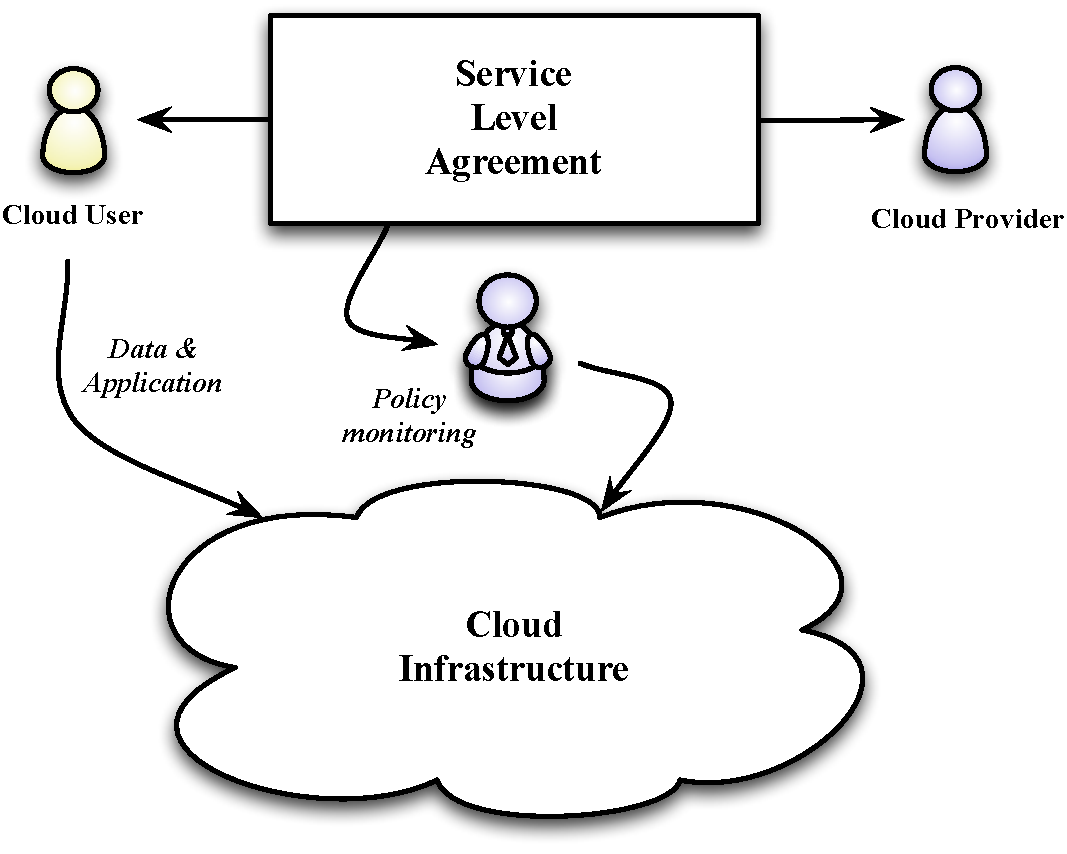
\includegraphics[scale=0.4]{Overview.pdf}
\caption{Usage management in existing cloud environment.}
\label{fig:overview}
\end{figure}

A natural consequence of static or hardwired handling of usage policies is that it prevents incorporation of complex usage policies. In case of solutions that follow the ``one-size-fits-all'' model, users have a limited say or options to express data usage terms. Furthermore, such approaches leaves cloud users with little or no room for negotiation of usage terms with cloud providers. Another major disadvantage of such a static approach is that there does not exist an interconnection between policies and the cloud infrastructure. This means that usage policies are not actionable, and it is not possible to reason about them with respect to the capabilities and limitations of the underlying cloud infrastructure. The lack of reasoning capabilities leads to under-utilization of cloud resources. While this impediment is not a major issue when dealing with simple policies, under-utilization of resources can cause serious revenue loss for cloud providers as the number of users and complexity of policies increase. 

In order to address these concerns, it is necessary that usage policies be managed by means of a usage management framework that will operate over a distributed cloud infrastructure as shown in Figure~\ref{fig:cloud-umf}. In this figure, a  cloud user and a cloud provider negotiate a usage policy and the price associated with the policy in an automated manner via software agents. Existing negotiation frameworks such as the Java Agent Development Framework and the FIPA negotiation protocols can be used for this purpose~\cite{BePoRi:02}.  Next, the policy is represented in a machine-readable and machine-actionable form. A rich body of research in the areas of rights expression languages~\cite{ODRL-req,JaHe:08,XrML-spec}, usage control languages~\cite{PaSa:04,HiPrBaScWa:07}, and access control languages~\cite{BlPa:76}, for formal representation of various usage semantics exists that can be leveraged to this effect. The policy is then interpreted and enforced over a distributed cloud infrastructure making use of existing trusted computing platforms to provide a comprehensive usage management solution. Significant business opportunities become available if these SLAs are easily customizable, allowing for price differentiation and yield management. In order achieve this, a usage management framework operating over a distributed cloud environment needs to be developed that satisfies the following goals:

\begin{enumerate}
\item Fine-grained expression of usage policies that can be negotiated between cloud users and cloud providers. 
\item Seamless movement of data within the cloud and persistent enforcement of usage policies across different services, at all levels of virtualization, along all data transformations throughout the lifetime of data in the cloud. 
\item Actionable policies that enable automated interpretation, reasoning, enforcement, usage tracking and reporting vis-a-vis the underlying cloud infrastructure. 
\end{enumerate}

\begin{figure}[!t]
\centering
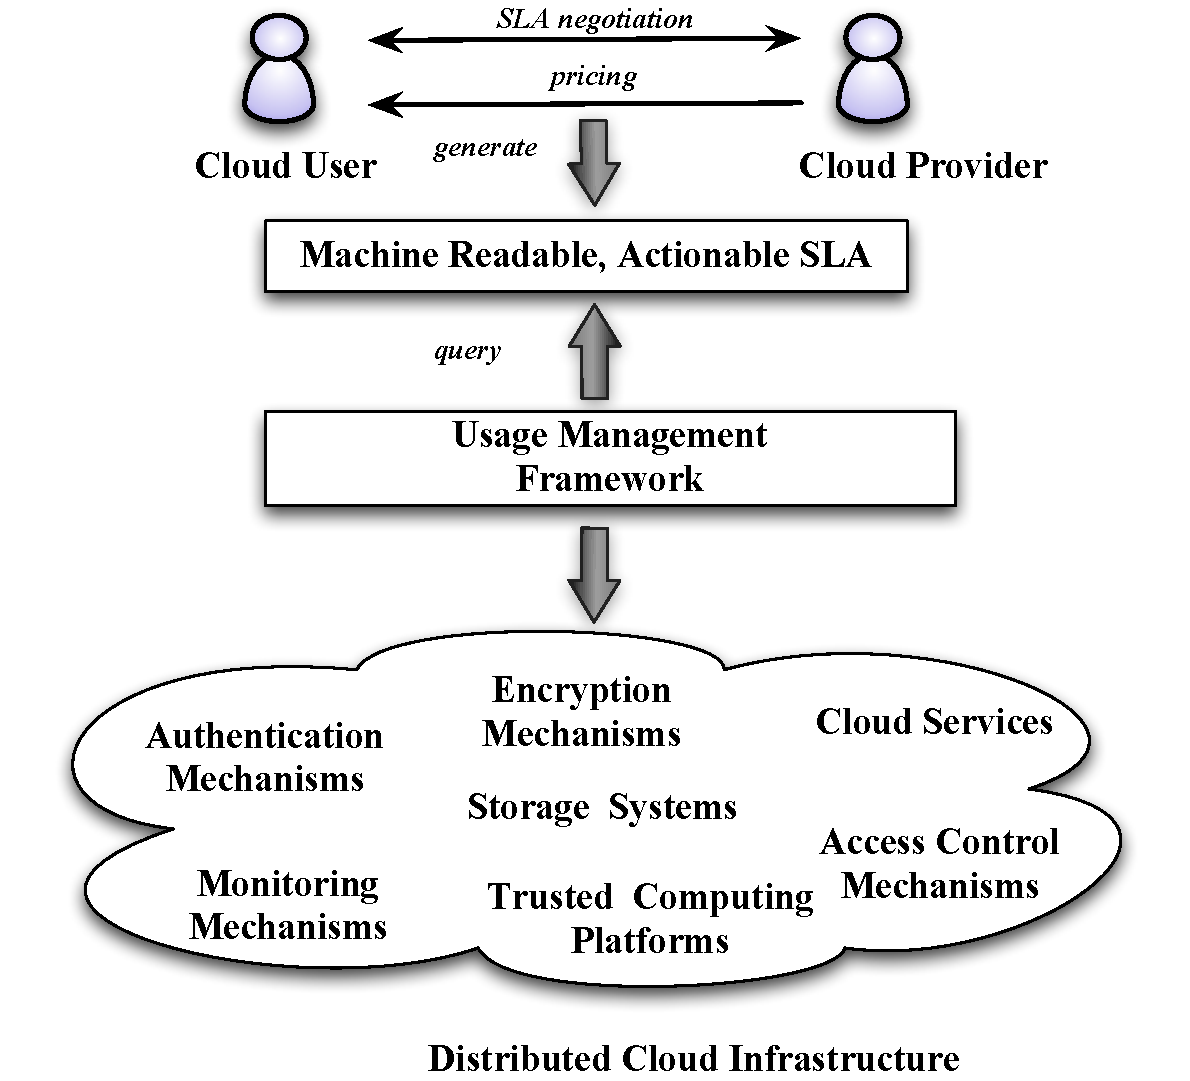
\includegraphics[scale=0.4]{cloud-umf}
\caption{Usage management in cloud.}
\label{fig:cloud-umf}
\end{figure}

The challenges presented by the specifics of a distributed cloud infrastructure in achieving these goals, and the features that such a framework must exhibit in order to address these challenges are discussed next. 

\begin{figure*}[t]
\centering
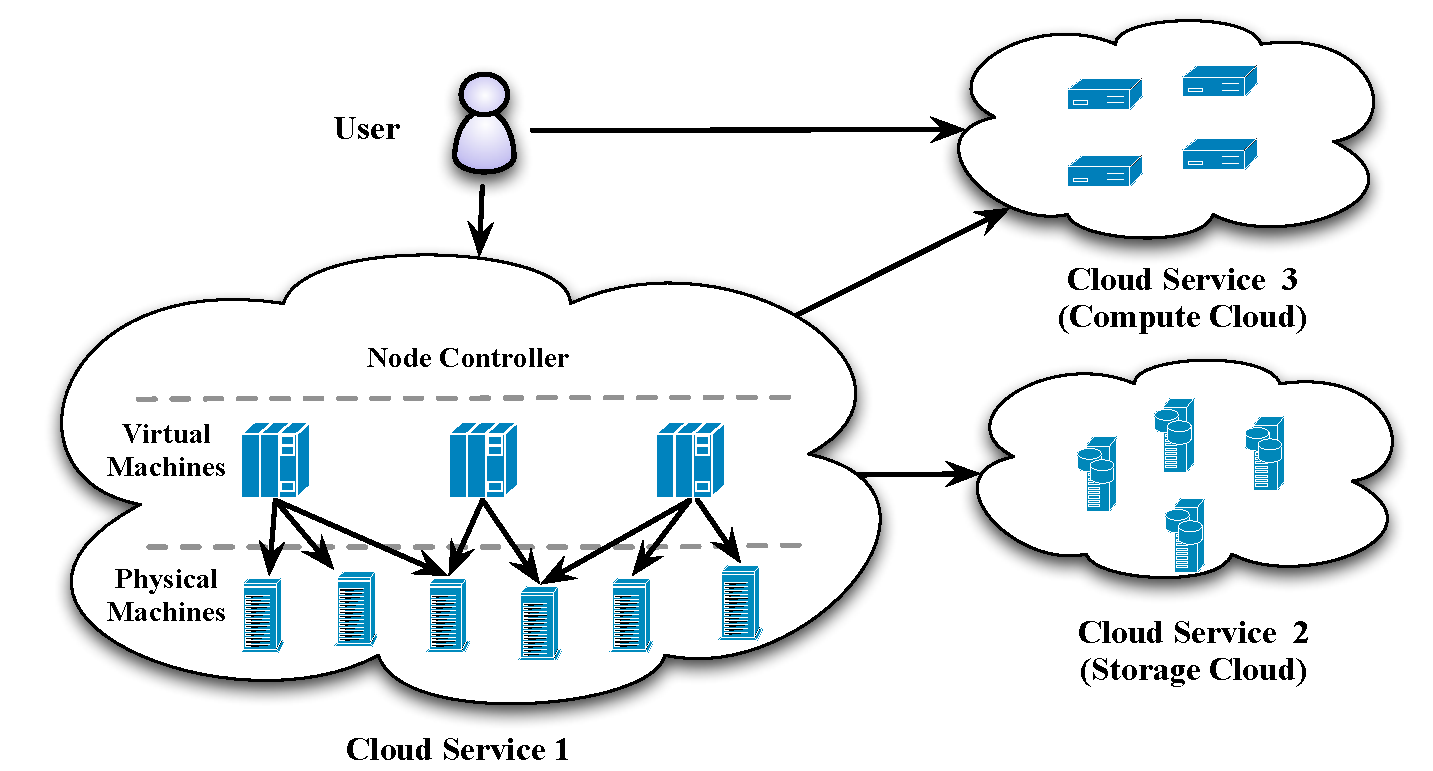
\includegraphics[width=14cm]{cloud-infra}
\caption{A distributed cloud infrastructure consisting of multiple cloud services and virtualization.}
\label{fig:cloud-infra}
\end{figure*}

\subsection{Challenges and Features}
A distributed cloud environment presents a unique set of challenges for the development of a framework that will enable usage management of data that are stored, routed and processed by different services operating within the cloud environment. Figure~\ref{fig:cloud-infra} shows the layout of a typical cloud computing environment. A distributed cloud environment may consist of one or more cloud services that are owned by different entities. Services are often composable, and available to users or other services via web-services technologies such as REST and SOAP.  The services provide virtualized resources to cloud users that are provisioned on demand to meet the SLA terms that are negotiated between the cloud provider and the user. Within a cloud service implementation, the set of virtual resources are mapped onto a distributed infrastructure of physical resources as shown in Figure~\ref{fig:cloud-infra}. The desired features of a usage management framework for clouds, discussed below, are based on this generalized layout of distributed cloud systems.

\subsubsection {An open interoperable framework}
In order to enable data from different cloud users to move seamlessly across different service providers, and leverage the use of existing security mechanisms, it is necessary to design an open usage management framework. The framework must provide a scaffolding upon which different technologies can be built, that can interoperate via standardized interfaces. In order to achieve this, it is necessary to identify focal points within the framework that need to standardized, and areas that should {\em not} be standardized to enable differentiation and innovation~\cite{BlCl:01}. 

In order for the usage policies to be consistently interpreted across different cloud providers, it is necessary to develop a common, extensible cloud ontology. All usage policies need to be developed using such a common cloud ontology.  There have been efforts towards the development of such an ontology, although not for the purpose of usage policy specification~\cite{YuBuDa:08}. 

Different cloud services will have different requirements as far as policy language characteristics are concerned. These characteristics  include expressive power, reasoning power, and ease of use. Development of  a single standard policy language that intends to satisfy all these requirements will be bloated, and difficult to formalize and reason over. Moreover agreement on a standard policy language will stifle innovation, and such a  language may be unable to address the needs of  future cloud systems. Hence the framework must accommodate coexistence of multiple languages that interoperate, and allow seamless movement of data within the cloud. However, existence of multiple policy languages have lead to serious problems with interoperability and user satisfaction in other fields such as DRM~\cite{JaHeMa:06}. To prevent this, rather than having each service provider understand every other policy language, policy interpretation, validation and reasoning need to be carried out via standard interfaces and a common ontology agreed upon by all cloud providers. Existing policy management frameworks for distributed systems can be used to address these concerns~\cite{JaHeLa:10,DaDuLuSl:01}. This approach, explained in the next section, will provide enough room for the existence of multiple languages, and will allow for incorporation of new languages. 

Figure~\ref{fig:sla-usage} shows how usage management needs to incorporated in existing SLA frameworks and resource allocation mechanisms. At every level in a cloud infrastructure where resource allocation takes place, the resource allocation process is over-ridden by data usage policy. This means, prior to allocation of resources,  resource allocation controllers must consult usage policies associated with the data for which resources are being allocated. 

\subsubsection{Dynamic interpretation}
Cloud computing services typically support a high degree of virtualization and dynamic composition of services. These two features have a different type of influence with respect to enforcement of QoS metrics and usage policy metrics. In the case of QoS metrics, enforcing the terms of the SLA agreement is solely the responsibility of the original cloud provider with whom the SLA is negotiated. Any other cloud services, engaged by the original cloud service provider to accomplish the task, have no responsibility towards respecting the original terms of agreement. In other words, QoS-based SLAs are brokered on a one-on-one basis, and have no bearing along the chain of servicing. 

On the other hand, usage policies need to be enforced by all service providers along the service chain that are a part of accomplishing the original task. For example if the original agreement mandates that the data cannot be stored in country $X$, then every cloud service along the chain which handles the data, must be capable of interpreting and enforcing this restriction. 

A cloud computing usage management framework must support dynamic interpretation of usage policies in order to enable usage policy enforcement across  service compositions and service chains. Dynamic interpretation allows policies to be expressed at a sufficient level of abstraction, and then interpreted appropriately depending on the particulars of a given cloud service environment~\cite{JaHeLa:10}. This ensures that usage policies are appropriately interpreted even if cloud users' data are passed on to cloud services with environments that are not known {\it a priori}. 

Another advantage of dynamic interpretation is that it takes into account the changes that occur within a given cloud service environment. This means that interpretation of a policy changes according to the changes that takes place in the cloud environment. For example, if the trusted computing base of a cloud service provider is attacked and becomes vulnerable, it allows the usage policies to be interpreted in a more strict manner after the attack. 

\begin{figure}[t]
\centering
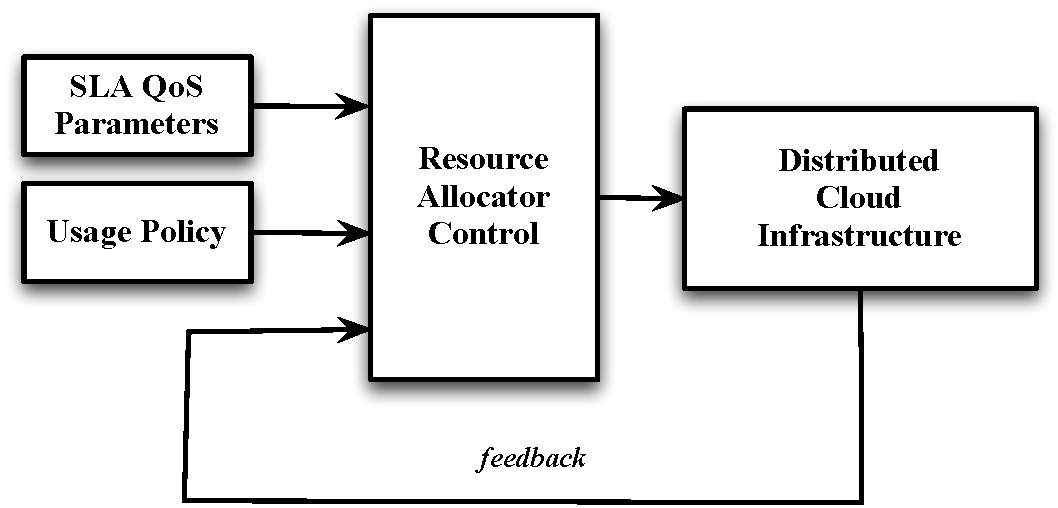
\includegraphics[width=9cm]{sla-usage}
\caption{Cloud usage management operating with SLA QoS monitoring.}
\label{fig:sla-usage}
\end{figure}

\subsubsection {Persistence}
In a cloud environment, data from multiple users may be handled by multiple cloud providers, and fractions of data sets may be stored, processed and routed across a geographically distributed computing infrastructure. Data are often subject to different types of transformations, aggregations and separations.  In such scenarios, it is necessary that all elements of a particular data set, associated with a given usage policy, are handled throughout their lifetime in the cloud, by different cloud services, in a manner that is consistent with the usage policy over the original data set. 

Usage management persistent across data aggregations is shown in Figure~\ref{fig:dynamics}. The service provided by Cloud Provider 1 aggregates multiple data form different sources, and feeds them to a service provided by Cloud Provider 2. In this scenario, each of the original data sources are governed by their own usage policies. After they are combined, the aggregated data set is governed by a combined usage policy that is a logical combination of the original two usage policies. Existing policy languages that support these combinations of policies may be used for this purpose~\cite{JaHe:08a}.

Enabling persistence in usage control requires the use of sophisticated naming, resolutions and policy manipulation mechanisms. It is necessary that in such scenarios, as data sets undergo transformations such as aggregation or separation, corresponding identifiers are created for the new data set, policies for the new data set are generated, and the new policies are attached to the corresponding data set. The policies may either by physically attached to the data set by means of encodings, or they may be attached via indirection. 

\begin{figure}[!t]
\centering
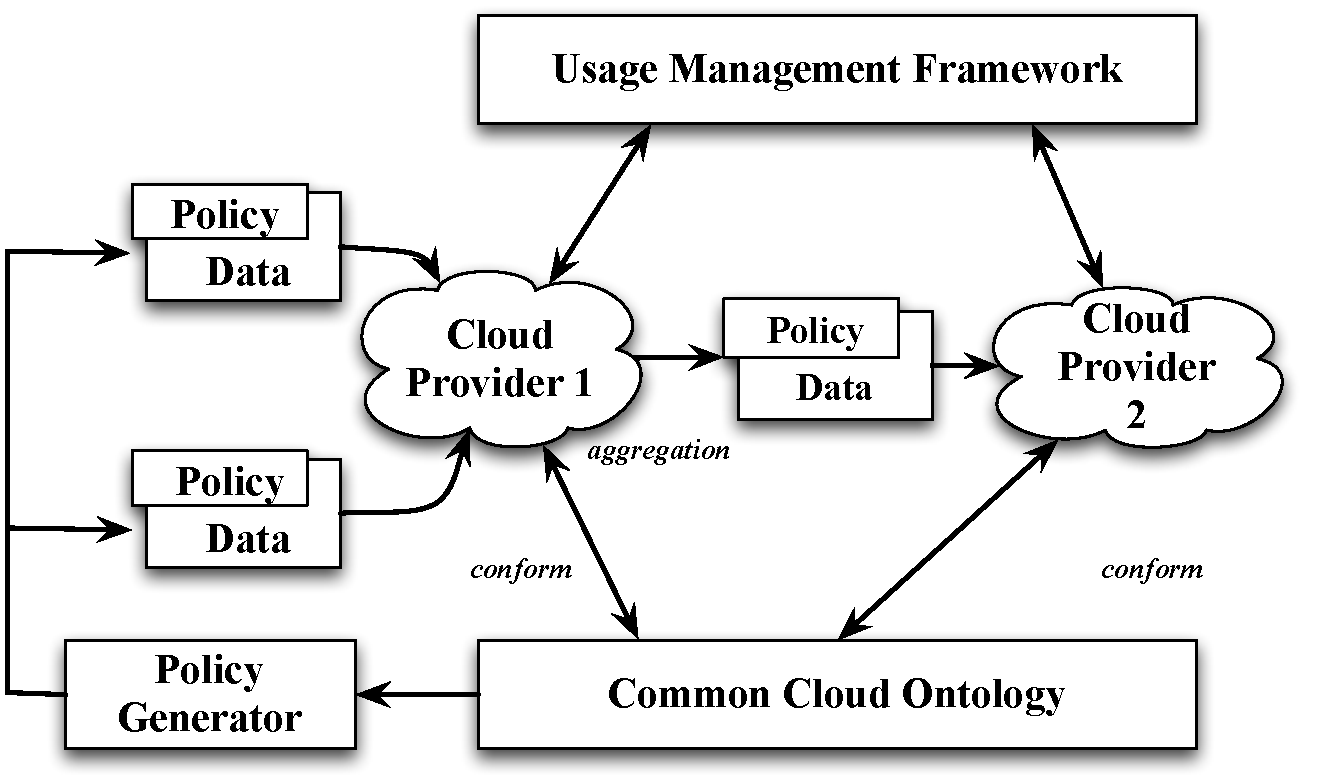
\includegraphics[scale=0.4]{dynamics}
\caption{Persistence of policies across data aggregations.}
\label{fig:dynamics}
\end{figure}

\subsubsection{Policy and cloud infrastructure interconnection}
It is important that usage management mechanism in cloud computing allows to reason about usage policies with respect to the capabilities of the underlying cloud infrastructure. It must be possible for a cloud provider to determine in an automated manner what aspects of a usage policy can and cannot be enforced, the reasons for not being able to enforce a particular usage policy, and the overhead cost involved in enforcing a usage policy. These questions can answered in an automated manner only if policies are expressed in a formal way that can be reasoned over. 

The usage management framework must also enable service providers to leverage existing security services such as encryption mechanisms, trusted computing base, authentication mechanisms, naming and resolution mechanisms, trust management mechanisms, negotiation frameworks and existing SLA frameworks to provide comprehensive security solutions in the cloud computing arena. The framework must provide hooks that enable use these mechanisms to enforce usage policies. 

In the next section a preliminary architecture that will form a platform upon which an open interoperable usage management framework for cloud computing can be built is proposed. The architecture enables use of multiple usage policy languages across different cloud providers while allowing interoperability among them. 

\section{Proposed Architecture}\label{sec:architecture}
In this section a preliminary architecture for usage management in cloud computing is described. The proposed architecture is based on the goals, principles and features discussed in the previous section. The architecture builds upon the previous work usage management in distributed environments~\cite{JaHeLa:10}.  The operation of the proposed architecture is divided into two phases, namely, a Setup phase and a Working phase. The Setup phase deals with the agreement on a usage policy and the setup of the cloud environment, and the Working phase deals with interpretation and enforcement of usage policies. The proposed architecture is currently being implemented in Ruby on Rails web application framework, and provides a web interface supporting functions for expression of policies, registration of policies, interpretation and evaluation of policies, among others. The details of the architecture are described below.

\subsection{Setup Phase}
The underlying principle driving the design of proposed architecture is that policies are evaluated within a context, and a context is separated form the syntax and semantics of policy languages. A usage policy consists of restrictions over usage expressed in terms of  context properties.  A context provides a formal representation of the cloud environment within which a policy is interpreted. A context formally represents the entities within the environment, the relations among the entities, properties of the cloud environment, and the current state of the environment. 

\begin{figure}[t]
\centering
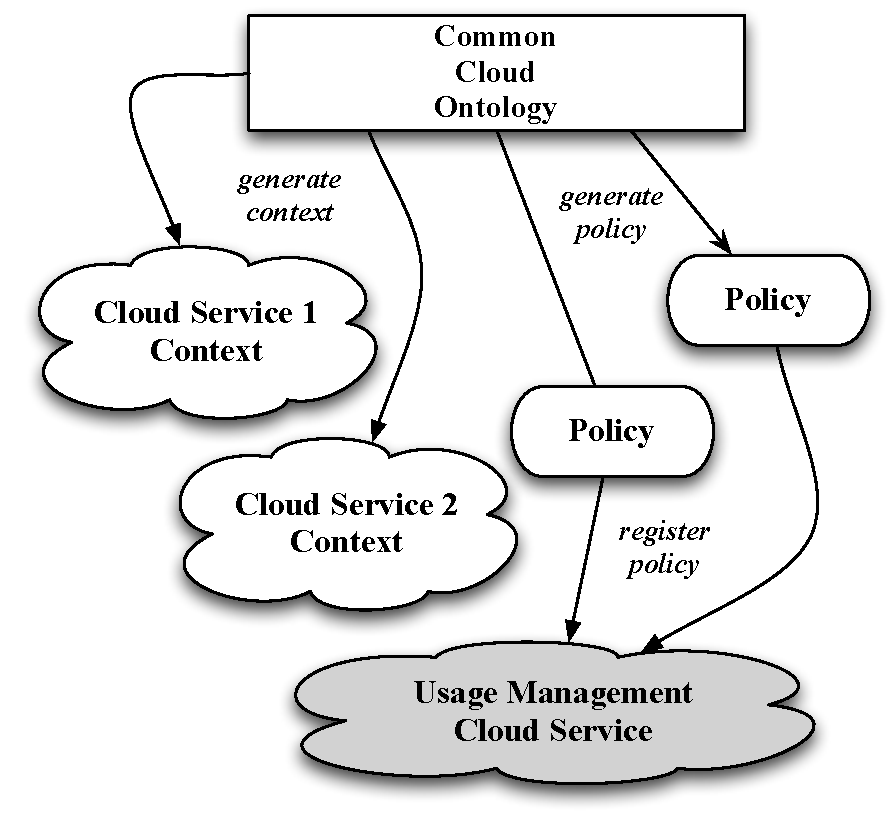
\includegraphics[width=9cm]{cloud-setup}
\caption{Setup phase usage management that include context and license generation.}
\label{fig:cloud-setup}
\end{figure}

\begin{figure*}[!t]
\centering
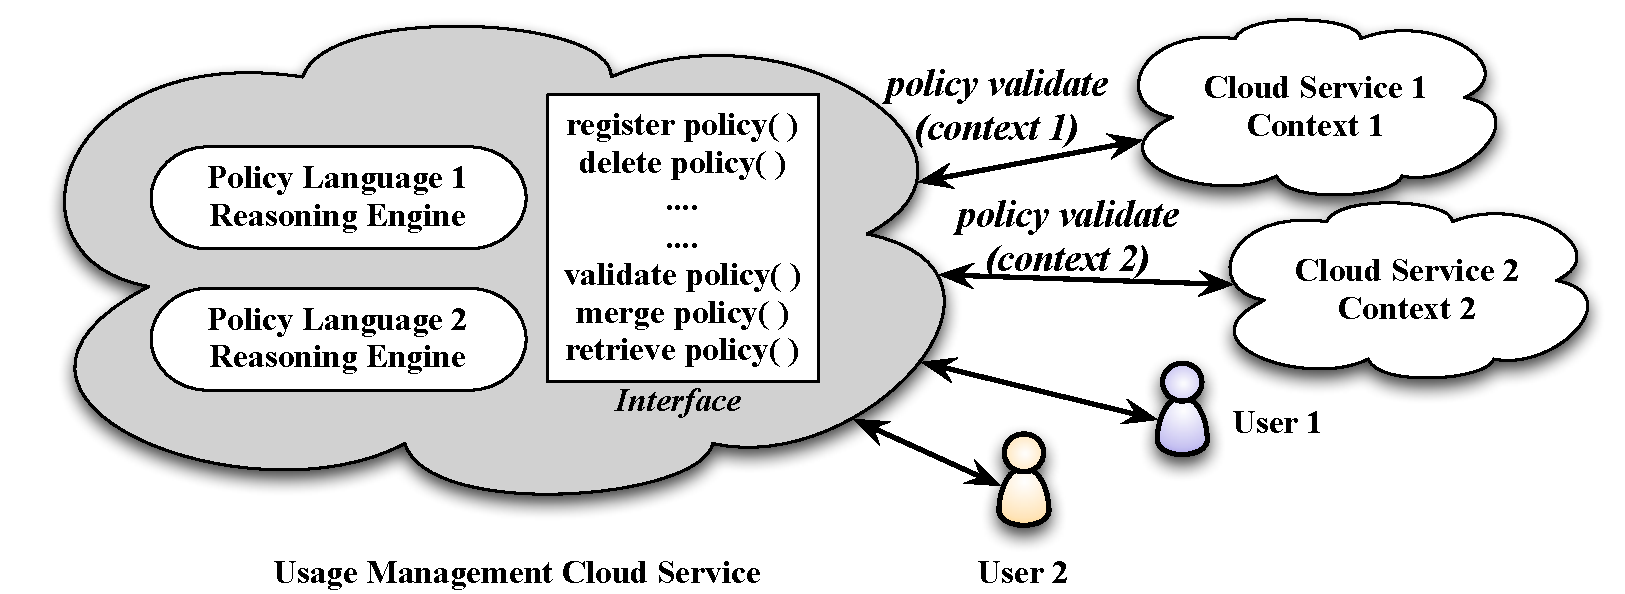
\includegraphics[width=13cm]{cloud-working}
\caption{Operation of usage management in cloud environment.}
\label{fig:cloud-working}
\end{figure*}

As an example, consider a context for a cloud service consisting of  different data processing sub-services ({\em dps}). A simplified context may consist of the following parameters: $\{date, dps\_location, dps\_trust-level \}$, where $date$ represents the global date, $dps\_location$ represents the location of the sub-service, and $dps\_trust-level$ represents the trust level of the sub-service ranging form 1-5. Usage policies for the data are then expressed as restrictions over these parameters. For example, a rudimentary usage policy might state that {\em `` Data set X can be processed only by a $dps$ located in the USA, with trust levels greater than 4, and not beyond December 16th, 2013''. }

Even though the example presented above is oversimplified, the point to note is that every cloud service has a representative context whose state (values taken by the parameters in the context) is continually maintained with appropriate values. During the Setup phase, shown in Figure~\ref{fig:cloud-setup}, cloud services define and generate their own context from a common cloud ontology that is shared among all cloud services. Depending the type and nature of cloud services, services will share certain common context parameters such as time, date and location, whereas differentiate in terms of other parameters. Usage policies over users' data set are generated using the common cloud ontology. It can be seen that all the parameters, using which policy restrictions are described, must be well-defined in the context of the cloud environment within which the policy is to interpreted.

In the proposed architecture, the policy languages used for expressing the policies are not standardized. Different cloud services may use their choice policy languages depending on their expression and reasoning requirements. However, in order for policies to be interpreted across different cloud environments, it is necessary that all policies make use the terms defined in the common cloud ontology that is shared by all cloud services. The manner in which policies are interpreted in the operational phase is explained next. 

\subsection{Working Phase}
The Working phase consists of policy management, policy interpretation and validation via a common usage management cloud service that is shared by different services within the cloud. The operation of usage management cloud service is shown in Figure~\ref{fig:cloud-working}. Instead of standardizing a common policy language for all cloud services, in the proposed architecture, the usage management cloud service provides a standard web interface for managing policies. This standard interface allows policies to be registered, retrieved, attached to data sets, deleted, validated, interpreted, reasoned, and merged with other policies by different cloud services via an extensible web interface. 

In the proposed system, usage policies are validated by cloud services in the following manner. Cloud services query the usage management service for a particular action on a particular data set by providing the context under which the action is intended to be carried out. The usage management service then evaluates whether the policy and the context are interoperable by comparing the terms. If the terms are consistent, then the policy restrictions are evaluated with respect to the current state of the context provided. If the restrictions are satisfied, the action is given a go ahead, otherwise it is denied. Every policy maintains a state or history of the usage performed by different cloud services on the data set. Such a history is commonly maintained in usage control and DRM languages to enforce count limits or obligation semantics on certain actions over a data set. Data usage histories can also be potentially used to validate data use with respect to policy terms, and provide cloud users with usage tracking services for their data.

Cloud services can register policies expressed in different policy languages,  however, all the policies are queried by means of a standard web interface. This approach ensures that the syntax and semantics of different policy languages is hidden from the cloud services that need to query usage policies. This precludes the need for every cloud service provider to deploy an interpreter for different policy languages. In addition, a service provider can introduce a new policy language for its operations, along side its previous policies expressed in the old policy language in a seamless manner. Figure~\ref{fig:cloud-working} shows how multiple policy languages can operate behind a common, standardized web interface for usage policy management.

\subsection{Single Provider Feedback System}\label{sec:single}
Controllable cloud systems enable providers to supply more closely targeted, cost effective services while at the same time providing service consumers with the confidence that the data and other artifacts their systems use are protected.  With that as our eventual goal, we first begin with a simple system managing currently accepted QoS parameters - system attributes like bandwidth, system memory allocation, and the like.  Specifically, we intend to provide the ability to monitor and control a virtual system hosted on a cloud infrastructure so that response time for a hosted application falls within a specific range of accepted parameters.

In order to manipulate a system to meet a preselected threshold of performance metrics, we must have access to measurement information with respect to factors affecting those metrics and we need to be able to adjust system performance in response to those measurements.  An example is system response time measured at the edge of the cloud provider's infrastructure as the metric we wish to control.  We could very well adjust system performance to meet that metric by manipulating the number of processing nodes, bandwidth available to those nodes, and node RAM allocations.

We have identified the attributes we wish to control.  This leads us to a group of requirements we can use to assemble a logical system architecture.  Requirements we know we need to address include:

\begin{itemize}
\item \textit{Performance:} We will be adjusting a system within specific soft real-time frames.  Ergo, we need to be able to collect feedback measurements, process those measurements, and make decisions about how to respond to those measurements quickly in order to avoid falling out of compliance with any performance parameters to which we must adhere.
\item \textit{Accessibility:} In order to control component systems, we must be able to access those systems.  In order to do so within time constraints, we must be able to access those systems electronically as well; physical access requirements simply will not scale into this performance domain.
\item \textit{Controllability:} We must be able to access the appropriate control primitives on the systems we need to tune.  This will include accessing compute node generation and termination capabilities.  It would help if we could access node performance information and tune those nodes as well, though this is not required; we can emulate this by terminating nodes in one configuration and creating nodes with another to more adequately address performance needs.
\end{itemize}

These system attributes lead us to a system architecture that is beginning to look like a traditional feedback-centric controllable system.

\begin{figure}[!t]
\centering
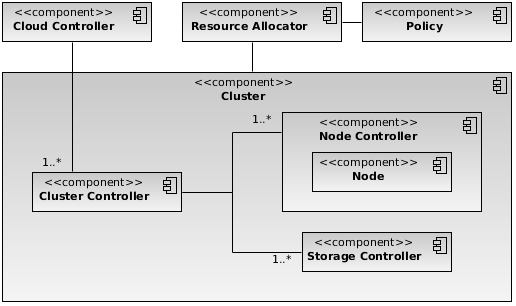
\includegraphics[width=3in]{Single-QoS}
\caption{Single Cloud Provider, Quality of Service.}
\label{fig:single-qos}
\end{figure}

The system shown in Figure \ref{fig:single-qos} has seven primary components.  These components work together to provide cloud services to consumers in a hypothetical infrastructure-as-a-service scenario.  This particular view addresses logical, functional components of this kind of a system rather than specific technologies used in an implementation, although some components are loosely modeled on popular open-source cloud environments (i.e. Eucalyptus).

Essentially, we have a cloud controller element that initiates provisioning of compute nodes within a given cluster. The cluster itself is managed by a cluster controller, which in turn controls storage controllers, node controllers, and by extension, nodes.  The nodes and node controllers themselves are monitored by a Resource Allocator which refers to a set of QoS requirements.

\begin{itemize}
\item \textit{Cloud Controller:} Provides an initial interface to administrative users to control the cloud.
\item \textit{Cluster Controller:} Managed by the cloud controller, the cluster controller manages the resources of a single cluster. A given cloud may contain multiple clusters.
\item \textit{Storage Controller:} Provides storage of system images and for other general storage needs.  This controller component is highly I/O sensitive.
\item \textit{Node Controller:} Responsible for allocating, delivering, and managing individual compute nodes upon which client software runs.
\item \textit{Node:} The compute node delivering services to end users and managed by the cluster's control infrastructure.  This is the primary computational resource accessed by users accessing managed cloud resources.
\item \textit{Policy:} Quality of service terms the cloud provider has agreed to honor for the cloud customer with respect to system delivery, provisioning, and overall performance.
\item \textit{Resource Allocator:} The component responsible for real-time tuning of the cloud system to maintain defined quality of service.
\end{itemize}

Operationally, the initial commands required to initialize the cloud are delivered from the \textit{Cloud Controller} to the \textit{Cluster Controller}, which then propagates another, related set of commands provisioning an initial set of resources from the \textit{Node Controllers} and the \textit{Storage Controllers}.  At this point, the initial system has been configured and is running, serving hosted software to its customer base.

Once the system is running, state data describing the performance metrics of interest is dispatched from \textit{Nodes} on the \textit{Node Controllers}, the \textit{Node Controllers} themselves, and the \textit{Storage Controller} to the \textit{Resource Allocator}.  The \textit{Resource Allocator} then processes this new event data in the context of the defined \textit{QoS} parameters.  This processing, in this model, is likely to be simple processing over the current event package or perhaps the current and the otherwise most recent event package.  This evaluation is very performance sensitive; we need to process the state of the current system quickly and adjust resource allocation accordingly.  Because of this soft real-time requirement, we do not have the luxury of spending significant time reviewing trending or providing sophisticated analysis over delivered event information.  Note that extension of this system into the feedforward domain would allow this kind of more robust system management, allowing us to employ more complex and powerful machine learning or neural systems to predict system needs.

Finally, if needed the \textit{Resource Allocator} will dispatch messages to the \textit{Cluster Controller}, \textit{Node Controller}, \textit{Nodes}, and \textit{Storage Controller} adjusting system profiles to ensure they remain within acceptable performance ranges.

\begin{figure}[!t]
\centering
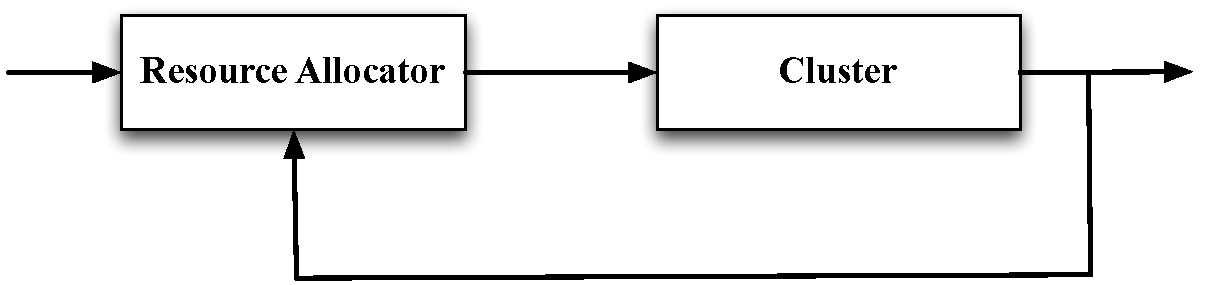
\includegraphics[width=3in]{feedback}
\caption{Control System Perspective.}
\label{fig:feedback}
\end{figure}

As shown in Figure \ref{fig:feedback}, we have an initial reference input reflecting the control parameters outlined by the \textit{Policy}.  The \textit{Resource Allocator} then processes both the reference input as well as system feedback metrics, providing control stimulus to the cloud cluster as output.

Note that in this example we are controlling the cluster.  Similar control loops exist over individual physical servers within the cluster, individual racks of servers within a single cloud provider system, and the entire cloud system itself. The first two control loops, the \textit{physical loops}, could control attributes like power consumption.  The latter example, the \textit{service loop}, allows a single provider to reason over groups of different customer SLAs under resource constrained conditions to determine which SLAs can be broken to minimize financial impact or prevent SLA breach; this allows for more efficient over-subscription of resources.

This control infrastructure as it has strict timing requirements with respect to event collection, analysis, and control, likely needs to be hosted in close physical proximity to the controlled systems.  Otherwise, the systems themselves can be located just about anywhere accessible to the Internet.  These logical components are not necessarily all hosted on physically distinct systems either, though generally at least the \textit{Storage Controller} and the \textit{Node Controller} are as they have remarkably different requirements with respect to processing power and I/O throughput.

Clearly, both the cloud service consumer and providers are impacted by this kind of infrastructure.  Consumers have systems performing within required performance bounds while providers are no longer required to maintain as strict administrative over-watch of managed systems.  This kind of system may also impact system developers, as dynamic node control and allocation imparts new requirements with respect to intra-system data handing and processing.  Generally however, accepted service development guidelines with respect to statelessness and allowing running processes to terminate prior to node shutdown will alleviate these issues.

When implemented, this kind of system will provide dynamic runtime control of cloud systems enhancing provider and customer confidence in the hosted infrastructure's performance potential.  This can also be extended into the usage management realm with more specific requirements with respect to how customer artifacts are managed, not just delivered.

\subsection{Single Provider Feedback System with Usage Management}\label{sec:singleUm}
Now that we have developed a cloud system capable of fairly granular control via a feedback control loop using QoS parameters, we will next incorporate specific usage management parameters.  In order to provide control over customer data artifacts in a cloud environment, we will adopt the system developed in Section \ref{sec:single}.  Our usage management control system must fit within the functional confines of the QoS system from Section \ref{sec:single} while extending the QoS functionality to artifacts not generally controlled via traditional QoS metrics.  For these purposes, a good example of an artifact not generally controlled via QoS parameters could be streaming network data.  While bandwidth throttling is clearly in the QoS domain, more specific uses of that data stream like caching and routing are not.   

Using a data stream as an example, we recognize some situations we clearly need to be able to control.  In this example, we will limit ourselves to a data stream emitted from a \textit{Node} on a \textit{Node Controller} which is routed to a user as a result of a user request.  Here, we have control over stream creation.  We want to limit the ability to update that data stream, we certainly do not want that stream deleted, and we want to limit who may read that stream.  In fact, we can safely assume in this scenario that update and deletion are operations we want to completely forbid, while we may want to limit stream readability, leading us to the primary extended requirement when adding usage management over a network stream in this case:

\begin{itemize}
\item \textit{Accessibility:} Data streamed through the cloud system must be able to be monitored and the accessibility of that stream needs to be dynamically tunable.  This implies that we need to be able to control routing and caching of all streaming data according to user specified conditions.  This also implies that we need to be able to control exactly which \textit{Node Controllers} are able to spawn which \textit{Nodes}.
\end{itemize}

\begin{figure}[!t]
\centering
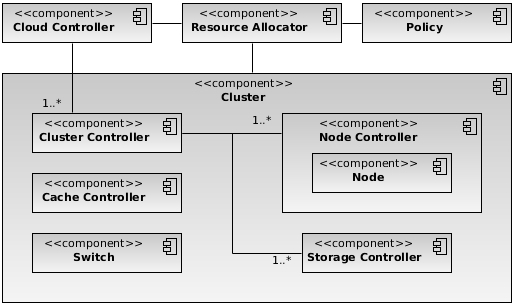
\includegraphics[width=3in]{Single-UM}
\caption{Single Cloud Provider, Usage Management.}
\label{fig:single-um}
\end{figure}

The addition of these attributes and requirements give us the logical system shown in Figure \ref{fig:single-um}.  The new system has new associations and components required to implement the degree of control required to limit the accessibility of the network stream.  We have added \textit{Cache Controllers} and \textit{Switches}, defined as:

\begin{itemize}
\item \textit{Cache Controllers:} Streaming network data, specifically media-centric streams, can and are cached by strategically located cache systems.  In order to control the read access of network data, we must be able to exercise explicit control over any caching systems in our infrastructure.
\item \textit{Switch:} Really any kind of hardware that controls the delivery of network data.  This component includes switches and routers primarily.  In order to control how data is accessed we must be able to control the locations to which it is delivered.
\end{itemize}

We have also added a new relationship to enable control over the \textit{Cloud Controller}.  To ensure that we can control where data is at any given time, we must also be able to control the geographic areas from which data is generated, especially if the virtual compute cloud spans national boundaries.

This again forms a controllable feedback loop, though one that is more complex than the simple QoS case.  The addition of new controllable items and relationships increases the responsibility and complexity of the \textit{Resource Controller} as new logic and capabilities are added to facilitate measurement and control of the larger system.  At this point however, the number of elements of complexity is still increasing linearly, leading us to believe that the problem may in fact still be tractable.

\subsection{Scaling to Multiple Providers}\label{sec:multiple}
We have briefly examined a single case controlling quality-of-service parameters and a second single case with quality-of-service and usage management parameters.  Moving from the first case to the second did increase the complexity of the problem somewhat, but not significantly.  Now we will expand our scope to multiple cloud providers, as shown in Figure \ref{fig:multiple}.

\begin{figure}[!t]
\centering
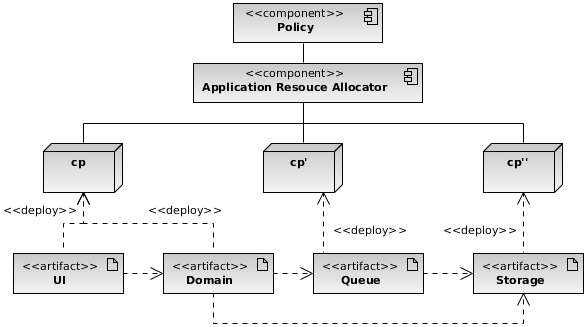
\includegraphics[width=3in]{Multiple}
\caption{Multiple Cloud Providers and hosted application.}
\label{fig:multiple}
\end{figure}

We now have three different cloud providers and various system layers of a sample application mapped to those providers.  The first provider, $ cp $, provides hosting for the \textit{User Interface} and \textit{Domain} layers.  The second provider, $ cp' $, provides queuing services to the application, while the third and final provider, $ cp'' $, provides data storage.  Each cloud provider contains the same elements contained by the providers in the previous sections, including a \textit{Resource Allocator} specific to that cloud provider.

Also, we have a new \textit{Resource Allocator}, an \textit{Application Resource Allocator}.  This new controller is required to provide control over the resources from the application's perspective.  The provider allocation controllers are sufficient for providing control over cloud specific resources from the provider's perspective, but cannot provide the appropriate view into the needs of the application as the application's needs span provider controller domains. As a result, we need a new controller element able to take a holistic, end-to-end view of the applications component systems that can then tune those systems so that application performance is effectively managed.  This effectively gives us a hierarchy of \textit{Resource Allocators}, each dedicated to optimizing a particular combination of resources, ranging from application-centric resources to provider-centric resources or other dependencies.

Here, we have a simple representation of a composite cloud system, a true system-of-systems, in the application implemented on the various cloud providers.  Furthermore, we now have the beginnings of an exponential problem with respect to \textit{application} control.  The complexity of a cloud provider may increase linearly, but the number of possible combinations of tunable parameters is exponential in the number of component systems, hinting at the beginnings of a potentially intractable problem.

\section{Conclusions and Future Work}\label{sec:conclusions}
In this paper we introduced the notion of usage management in cloud computing environment. Cloud computing exhibits a unique set of characteristics that require usage management of users' data according to user concerns and expectations. We analyzed the challenges involved in the design and development of a framework for usage management in cloud environments. We showed that such a framework needs to be open to leverage existing security technologies and SLA frameworks. The framework needs to exhibit features such as support for multiple policy languages, existence of a common cloud ontology, dynamic interpretation and persistence of usage enforcement. Finally a preliminary framework that supports multiple policy languages was introduced that provides a platform upon which such a framework can be built. 

Future work involves efforts towards the development of a common extensible cloud ontology that will provide a common vocabulary for cloud environments and enable interoperability. Such an ontology needs be developed by taking into consideration the requirements of different cloud services. In addition, it is necessary to standardize interfaces for other security mechanisms mentioned in the paper that can be incorporated within the framework. Finally, existing policy languages can be modified to be incorporated within the framework, and new ones need to designed to address the specific needs of different cloud services. 

\bibliographystyle{Plain}
% argument is your BibTeX string definitions and bibliography database(s)
\bibliography{drm}
\end{document}